\section{Experiments}\label{sec:experiments}

The experiments evaluate whether BotRHG improves social bot detection and how its key components affect performance. We first describe the experimental setup, and then present the main comparison, component analysis, hyperparameter sensitivity, and a case study.

\subsection{Experiment Setup}

\paragraph{Datasets.}
We use two public social bot detection benchmarks, TwiBot-22~\cite{twibot22benchmark} and TwiBot-20~\cite{feng2021twibot20}. TwiBot-20 contains 5,237 human accounts, 6,589 bot accounts, 229,580 nodes, and 227,979 normalized social edges; we adopt the standard setting in~\cite{feng2021twibot20}. For TwiBot-22, we conduct evaluation on a fixed sampled subset. The subset is sampled within the released train/validation/test splits and is kept identical for all compared methods. It contains 11,542 labeled accounts, including 1,575 bots and 9,967 humans, together with 128,095 social edges.

\paragraph{Baselines.}
Baselines cover four representative groups. Feature-based methods include BotHunter~\cite{bot_hunter2018} and FriendBot~\cite{friendbot2020}. Graph-based and multimodal detectors include BotRGCN~\cite{feng2021botrgcn}, RGT~\cite{feng2022rgt}, BIC~\cite{lei2023bic}, BotMoE~\cite{liu2023botmoe}, and SEBot~\cite{yang2024sebot}. We also compare with BotBR~\cite{lin2025botbr}, a reliability-oriented detector, and LMBot variants~\cite{cai2024lmbot} for graph-knowledge distillation and graph-less inference.

\paragraph{Evaluation metrics.}
Following prior studies~\cite{feng2022rgt,yang2024sebot,gao2025higherorder}, we report Accuracy, Precision, and F1-score. Precision and F1-score are macro-averaged. In the result tables, bold and underlined values indicate the best and second-best performance, respectively.

\paragraph{Implementation details.}
For the main comparison, we report the mean and standard deviation over five runs. Ablation and hyperparameter sensitivity experiments are conducted on TwiBot-20 under a fixed random seed setting. All textual, profile, behavioral, and graph-based features are normalized using training-set statistics. The hidden dimension is set to 788, and the graph and hypergraph modules are configured with two layers. We perform grid search over the KNN support size $K \in \{4,8,16\}$, sampled fanout $\in \{32,64,128\}$, and routing budget $\beta \in \{5\%,10\%,20\%\}$, with $K=8$, fanout 64, and $\beta=10\%$ used as the default setting. Graph training runs for at most 200 steps with a GNN batch size of 512. We use AdamW for optimization, with learning rates of $1\times10^{-5}$ for the text encoder and $5\times10^{-4}$ for graph modules, and apply graph-side weight decay of $1\times10^{-5}$. The experiments are implemented with PyTorch, PyTorch Geometric, and scikit-learn, and conducted on a CentOS 7 server equipped with two NVIDIA GeForce RTX 3090 GPUs.

\subsection{Main Results}

Table~\ref{tab:main-results} compares the proposed detector with representative baselines. All main results are reported as the mean and standard deviation over five runs.

\begin{table}[t]
\caption{Main results on TwiBot-20 and sampled TwiBot-22. Values are reported as percentages. Bold and underlined values indicate the best and second-best results, respectively. A dash denotes unavailable compatible results.}
\label{tab:main-results}
\centering
\scriptsize
\setlength{\tabcolsep}{2.5pt}
\resizebox{\textwidth}{!}{
\begin{tabular}{m{2.2cm}|cccccc}
\toprule
Method & \multicolumn{3}{c}{TwiBot-20} & \multicolumn{3}{c}{TwiBot-22} \\
\cmidrule(lr){2-4}\cmidrule(lr){5-7}
 & Accuracy & Precision & F1-score & Accuracy & Precision & F1-score \\
\midrule
BotHunter~\cite{bot_hunter2018} & 75.28 $\pm$ 0.42 & 76.34 $\pm$ 0.51 & 74.39 $\pm$ 0.42 & 77.31 $\pm$ 0.19 & \textbf{78.56 $\pm$ 1.19} & 63.23 $\pm$ 0.31 \\
FriendBot~\cite{friendbot2020} & 77.19 $\pm$ 0.46 & 77.71 $\pm$ 0.46 & 76.63 $\pm$ 0.48 & -- & -- & -- \\
\midrule
BotRGCN~\cite{feng2021botrgcn} & 85.68 $\pm$ 0.57 & 85.88 $\pm$ 0.69 & 85.49 $\pm$ 0.55 & 72.21 $\pm$ 2.29 & 66.50 $\pm$ 4.57 & 60.55 $\pm$ 2.10 \\
RGT~\cite{feng2022rgt} & 86.39 $\pm$ 0.25 & 86.63 $\pm$ 0.26 & 86.20 $\pm$ 0.26 & 72.24 $\pm$ 2.38 & 64.40 $\pm$ 5.58 & 56.73 $\pm$ 6.91 \\
BIC~\cite{lei2023bic} & 85.55 $\pm$ 0.50 & 85.78 $\pm$ 0.53 & 85.34 $\pm$ 0.51 & \underline{78.56 $\pm$ 0.97} & \underline{74.33 $\pm$ 1.40} & \textbf{73.42 $\pm$ 0.95} \\
BotMoE~\cite{liu2023botmoe} & 86.12 $\pm$ 0.50 & 86.38 $\pm$ 0.66 & 85.92 $\pm$ 0.47 & 64.99 $\pm$ 1.60 & 65.62 $\pm$ 0.92 & 63.64 $\pm$ 1.36 \\
SEBot~\cite{yang2024sebot} & 86.29 $\pm$ 0.33 & 86.52 $\pm$ 0.31 & 86.10 $\pm$ 0.35 & -- & -- & -- \\
\midrule
BotBR~\cite{lin2025botbr} & \underline{86.91 $\pm$ 0.20} & 87.19 $\pm$ 0.21 & \underline{86.72 $\pm$ 0.21} & 76.09 $\pm$ 3.99 & 68.94 $\pm$ 17.60 & 60.34 $\pm$ 12.20 \\
\midrule
LMBot-GNN~\cite{cai2024lmbot} & 85.11 $\pm$ 0.39 & 86.44 $\pm$ 0.73 & 84.65 $\pm$ 0.39 & 74.98 $\pm$ 1.46 & 69.19 $\pm$ 2.42 & 64.29 $\pm$ 3.80 \\
LMBot-LM~\cite{cai2024lmbot} & 85.41 $\pm$ 0.10 & \underline{87.47 $\pm$ 0.57} & 84.87 $\pm$ 0.21 & 74.72 $\pm$ 1.27 & 69.46 $\pm$ 2.80 & 62.90 $\pm$ 2.25 \\
\midrule
\textbf{BotRHG} & \textbf{88.93 $\pm$ 0.53} & \textbf{89.18 $\pm$ 0.43} & \textbf{88.78 $\pm$ 0.48} & \textbf{82.41 $\pm$ 1.40} & 73.14 $\pm$ 1.34 & \underline{71.31 $\pm$ 1.04} \\
\bottomrule
\end{tabular}
}
\end{table}


Our method achieves the best performance on TwiBot-20 across Accuracy, Precision, and F1-score, outperforming the strongest baseline BotBR by 2.02, 1.99, and 2.06 percentage points, respectively. On TwiBot-22, it obtains the highest Accuracy and a competitive F1-score, ranking second to BIC on F1-score. These results show that BotRHG improves the standard TwiBot-20 benchmark and remains effective on the TwiBot-22 setting. FriendBot and SEBot are not included for direct comparison on TwiBot-22 because compatible results are not available under the same evaluation protocol.

Feature-based methods such as BotHunter and FriendBot rely heavily on handcrafted profile, content, and network statistics, and their performance is limited when bots imitate observable account attributes. Graph-based and multimodal methods, including BotRGCN, RGT, BIC, BotMoE, SEBot, and BotBR, exploit relational or heterogeneous evidence and generally perform better than feature-only baselines. However, they usually apply structural propagation or feature fusion uniformly. In contrast, our method uses a local reliability estimate for each account and introduces higher-order hypergraph evidence only through reliability-guided routing and selective residual correction, which helps preserve reliable base predictions while improving low-reliability accounts.

\subsection{Ablation Study}

To examine the contribution of each component, we construct four variants of the proposed model. \textit{w/o Reliability-Guided Routing} removes reliability-guided routing and applies correction without account-level reliability selection. \textit{w/o Residual Correction} keeps the routing stage but disables the selective residual correction module. \textit{w/o Hypergraph Correction} replaces hypergraph correction with a fine-tuned RoBERTa + RGCN variant, comparing the proposed design with a conventional graph detector. \textit{w/o Random Routing} randomly selects the same number of routed accounts under the same routing budget, replacing the routing induced by the local reliability estimate with random routing.

\begin{table}[t]
\caption{Ablation study on TwiBot-20. The full model uses $K=8$, fanout 64, and a routing budget of 10\%.}
\label{tab:component-ablation}
\centering
\small
\begin{tabular}{lcc}
\toprule
Variant & Accuracy & F1-score \\
\midrule
Full model & \textbf{0.8893} & \textbf{0.8878} \\
w/o Reliability-Guided Routing & 0.8850 & 0.8835 \\
w/o Residual Correction & 0.8774 & 0.8755 \\
w/o Hypergraph Correction & 0.8715 & 0.8684 \\
w/o Random Routing & 0.8698 & 0.8677 \\
\bottomrule
\end{tabular}
\end{table}


Table~\ref{tab:component-ablation} reports the fixed-seed component analysis on TwiBot-20. The full model achieves the best Accuracy and F1-score. Removing reliability-guided routing reduces F1-score from 0.8878 to 0.8835, indicating that reliability-guided routing helps identify accounts that benefit from additional correction. Removing selective residual correction causes a larger drop to 0.8755, suggesting that higher-order correction provides useful information beyond the base detector. The strongest degradations come from w/o Hypergraph Correction and w/o Random Routing, whose F1-scores fall to 0.8684 and 0.8677, respectively. These results suggest that the improvement does not come merely from adding graph capacity or correcting a fixed number of accounts; it depends on both selective residual correction and routing based on the local reliability estimate.

\subsection{Hyperparameter Sensitivity}

We examine three hyperparameters under the fixed-seed TwiBot-20 setting: the KNN support size $K$, the sampled fanout, and the routing budget $\beta$. Figure~\ref{fig:hparam-sensitivity} reports the results.

\begin{figure}[!htbp]
    \centering
    \includegraphics[width=.92\textwidth]{figures/twibot20_seed1_hparam_sensitivity.pdf}
    \caption{Hyperparameter sensitivity on TwiBot-20. The dashed line indicates the full-model setting: $K=8$, fanout 64, and a routing budget of 10\%.}
    \label{fig:hparam-sensitivity}
\end{figure}

For the KNN support size, the model performs best at $K=8$. A smaller support set may provide insufficient local reference evidence, while a larger support set may include weakly related accounts and dilute the reliability signal. For sampled fanout, fanout 64 gives the best result, and fanout 32 remains competitive, whereas fanout 128 leads to a clear performance drop. This trend indicates that expanding the sampled neighborhood can enrich structural context, but excessive expansion may introduce noisy or task-irrelevant relations. For the routing budget, $\beta=10\%$ achieves the best Accuracy and F1-score. A smaller budget may miss low-reliability accounts, while a larger budget routes more accounts whose base predictions are already reliable, increasing unnecessary correction.

\subsection{Case Study}

\begin{figure}[!t]
    \centering
    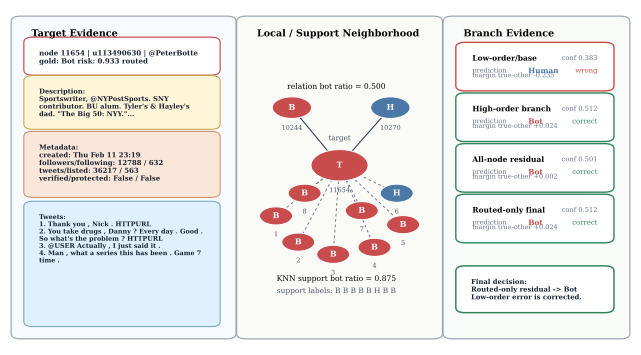
\includegraphics[width=.56\textwidth,trim=145 165 510 125,clip]{figures/casestudy.pdf}
    \caption{Case study for an initially misclassified routed account on TwiBot-20. Solid lines denote observed social neighbors, and dashed lines denote higher-order KNN links used for selective residual correction.}
    \label{fig:case-study}
\end{figure}

Figure~\ref{fig:case-study} presents a bot account that is initially misclassified as Human by the base detector. Its profile and tweet content do not exhibit clear bot-specific signals, and its observed social neighborhood contains both human and bot accounts, making the low-order prediction biased toward the Human class. After reliability-guided routing, the dashed KNN links associate the target account with bot-related reference accounts in the hybrid representation space and form a hyperedge. Selective residual correction then introduces additional higher-order evidence, increases the confidence toward the Bot class, and revises the incorrect prediction.
